% $  Id: related.tex  $
% !TEX root = main.tex


%%
\section{Background on \acl{ML} Techniques}
\label{sec:related}

This section provides the background for the main existing \ac{ML} techniques --that is, linear 
regression and neural networks. We present the main ideas behind each of these techniques, their 
application domains, and some of the technologies available to use each of them. 

%%%
\subsection{Linear Regression}
\label{sec:linear-regression}

Regression Models are used for the prediction of values in a continuous domain. Linear regression 
focuses on reducing making accurate predictions of data by reducing the error in every prediction 
step. However, in order to make data predictions, it is required to provide input examples to the 
model. Moreover, the accuracy of the predictions depends on the quality of input data, as the model 
creates data representations based on its input. this highlights the main characteristic of supervised 
learning models, as linear regression, which are focused on representation rather than code. The 
basic model for linear regression is shown in \fref{eq:linearReg}

\begin{equation} \label{eq:linearReg}
y'=w_I x_I+b
\end{equation}

where:
\begin{enumerate}
 \item Label ($y'$): is the desired output, for instance, the target the model is aiming for.
 \item Features ($x$):  are the way data is represented. Given that the user determines features, they are also referred to as the known input. Features take values on the index set $I$. 
 \item Weights ($w$): represent the search slope, which is the coefficient for the independent variable, that in this case is the corresponding feature.  Weights take values on the index set $I$. 
 \item Bias ($b$): is the offsets of the predictions made. 
\end{enumerate}

The linear regression model defines the relation between features and labels. That is, it maps 
input examples to predict labels. This is a recursive process where the model progressively learns 
the interrelation between features and labels. As a result the model resolves the appropriate weight 
and bias for all values from the given examples. 
Taking into account that users modify the model parameters, it is imperative to measure the difference 
between predicted values and obtained values.  A common way to identify the error is through the 
\emph{least square errors technique}. This error model is most appropriate to use when users begin 
to interact with \ac{SML} models, because the difference between an incorrect target and the original 
value will be made largely evident. Using this error model,  prediction errors in a single example will 
be easier to identify, and thus more apparent to improve and modify. \fref{eq:L2loss equation} shows 
the equation used to calculate the least square errors in the model.

\begin{equation} \label{eq:L2loss equation}
\displaystyle
S = \sum_{i=0}^n (y_i - h(x_i))^2
\end{equation}

In this model $h(x)$ represents the corresponding estimated value of $x$~\cite{rish15}.
The objective of the model is to reach the minimum loss; this goal is achievable through different 
approaches. In this paper we present only two of such approaches. The \emph{gradient descent} 
approach, is the derivate of the least square error result, and together with the weight and bias for a 
given example informs how loss changes for a given example. With this information, it is possible to 
adjust the model iteratively until learning weights and bias become as small as possible. 
The \emph{\ac{SGD}} approach, repeats the process of the gradient descent for each individual 
example.

\begin{equation} \label{eq:SGD}
(y - h(x))^2
\end{equation}

\fref{eq:SGD} shows the \ac{SGD} approach, in which the gradient is calculated one example at a 
time. As a result, initial values for the bias and weight are not relevant. However most of the time it is 
appropriate to begin with $0$ for both values.

Both gradient descent algorithms multiply the gradient by a scalar known as the learning rate 
(sometimes called step size) to determine the next prediction point. There are several variations to 
the \ac{SGD}, and in all of them it is possible to set the learning rate.  Moreover, the learning rate 
parameter tells the optimizer how to move the weights in the direction of the gradient for a mini batch. 
Having a low learning rate is decisive, because it provides a more reliable training, at the cost of 
having longer optimization time, as the steps towards the minimum loss of the function are especially 
small. If the learning rate is high it is possible that the training diverges rather than converging. 
Weight changes can become so big that the optimizer overshoots the minimum and makes the loss 
worse. The information presented before rises a new question: How can the modeler identify the 
correct learning rate for the process? 
As delusive as it might be, the first method with which one can select the correct learning rate is the 
Na\"ive approach. This consists of trial and error predictions. Start with any learning rate and from 
there begin to modify the learning rate according to the obtained results. 

\begin{figure}[htbp]
  \centering
  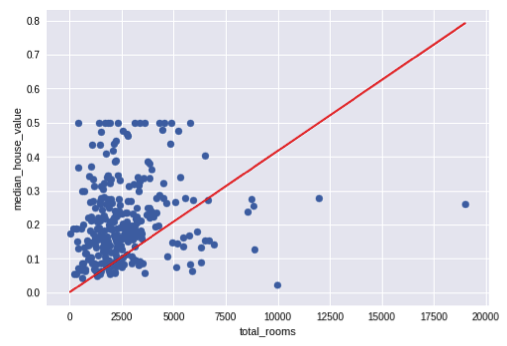
\includegraphics[width=0.8\textwidth]{images/linearGraph}
  \caption{ The results plotted in the graph suggest that there might be a better line, which fits more data, thus resulting in a prediction model that has a greater accuracy.}
  \label{fig:linearGraph}
\end{figure}

It is recommended to start with a large value such as 0.1 and from there exponentially lower the 
values (0.1,0.01,0.001).
~\citet{leslie15}, describes a second method, which consists of an initial low learning rate that is then 
increased exponentially when a new batch comes in.
The ideal learning rate in one-dimension is $\frac{1}{f(x)^n}$ (the inverse of the second derivate of 
$f(x)$ at $x$). The ideal learning rate for two or more dimensions is the inverse of the Hessian (the 
matrix of second partial derivates)~\cite{leslie15}.


%%%%
\paragraph{Applications}

Due to the simplicity of linear regression models applications revolve around prediction and are 
widely used in a broad set of domains (\eg business, economics, or medicine). That is to say that the 
best uses to linear regression supervised models are given when the goal is to analyze to obtain 
possible outcomes. As a matter of fact, this branch of \ac{ML} is appropriate for predictions regarding 
prices, such as real state or banking, estimating salaries and predicting enterprise areas performance. 
Other uses for this implementation include traffic prediction, recommending related products for 
clients, and determining medical recovery time~\cite{grandeur17}. As these examples show, a broad 
area of  problems can be solved using this model, Dr. Robin Hanson once quoted ``Good CS expert 
says: Most firms that think they want advanced AI/ML really just need linear regression on cleaned-up 
data.'' Moreover, this model is able to blend with more sophisticated techniques that provide more 
accurate results for the mentioned applications. 


%%%
\subsection{\acl{NN}}

\acl{NN} are a collection of parallel processors connected together in the form of a directed graph, 
organized such that the network structure lends itself to the problem being considered. Scientists 
studied human neurons and were able to identify that the impressive parallelism and interconnectivity 
observed in the biological systems account for the ability of the brain to perform complex pattern 
recognition in a few hundred milliseconds~\cite{freeman91}.

A biological neuron has three components important in the understanding of artificial neurons: 
dendrites, soma and axon. 
\begin{enumerate}
 \item Axon:  the region where a neuron sends messages to other neurons.
 \item Dendritic tree: the area where the neuron collects input from other neurons.
 \item Synapses: the region in which an axon from one neuron contacts the dendritic tree of another 
 neuron. A Spike of activity in the axon causes charge to be injected into the post-synaptic neuron.
\end{enumerate}
Summed up, electric impulses known as signals are transmitted through 
the synaptic gap by means of a chemical process. The action of the chemical transmitter modifies the 
incoming signal (typically by scaling the frequency) in a manner similar to the action of the weights in 
an Artificial Neural Network~\cite{fausett93}. When sufficient input is received, the cell fires --that is, it 
transmits a signal over its axon to other cells. 

\begin{figure}[htbp]
  \centering
  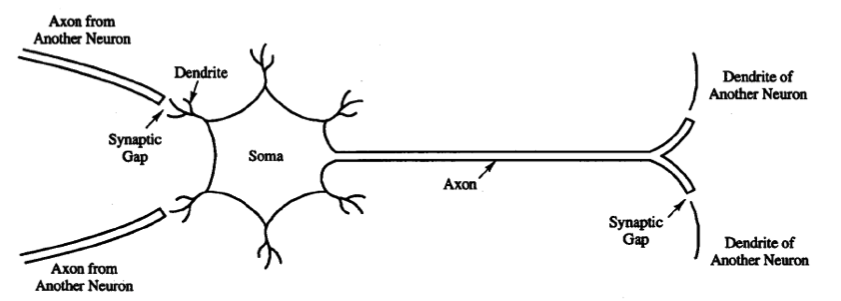
\includegraphics[width=\textwidth]{images/neuron}
  \caption{ Human Neuron diagram (taken from~\cite{fausett93}) }
  \label{fig:humanNeuron}
\end{figure}

According to this definition,  \ac{NN} comprise a system where biological neurons are represented by 
nodes and are considered a simplified representation of a processing element (unit). Additionally, 
connections between units are represented as edges. This is interpreted as the architecture of the 
model~\cite{fausett93}. As a way to indicate the information flow of the network arrowheads in the 
model represent connections between nodes. A \ac{NN} model is shown in \fref{fig:neuronNet}. 
Furthermore understanding the dynamics of the model 
is important to recognize how similar the \ac{ML} version is to the biological nervous system. As a 
matter of fact, humans are born with as many as 100 billion neurons that are not replaced when they 
die. As a reflection of this, \ac{NN} are designed to be insensitive to small damage to the network. 

When using \ac{NN} it is not necessary to handle correct algorithmically defined procedures that are 
able to take an input and represented in the correct output. Rather, for this type of models a 
collection of representative examples with the desired translation is needed. Progressively the model 
will adapt itself to return the desired output when presented with known inputs. As a results, \ac{NN}  
have the strong characteristic of finding its  own solution to particular problems based on gained 
experience. 

\begin{figure}[htbp]
  \centering
  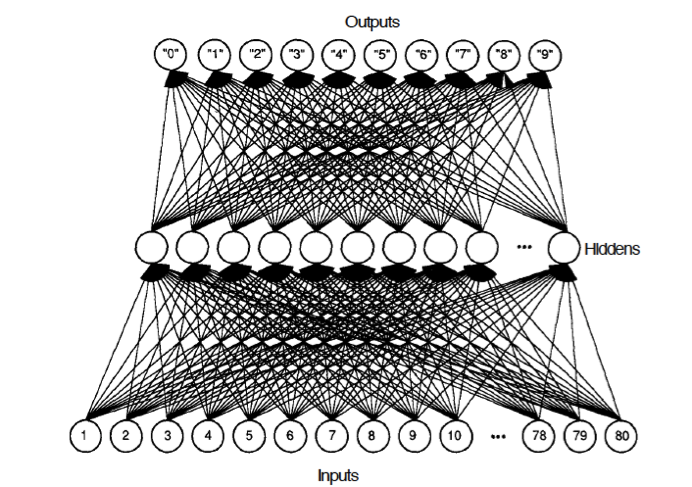
\includegraphics[width=\textwidth]{images/net}
  \caption{ Diagram of a \acl{NN} capable of identifying written numbers (taken from~\cite{freeman91}) }
  \label{fig:neuronNet}
\end{figure}

Neurons in these models can be classified according to the amount of detail and complexity of the 
inputs. Among these classifications one can find linear neurons, binary threshold neurons, rectified 
linear neurons, sigmoid neurons, and stochastic binary neurons. For the scope of this paper, a model 
comprised with linear neurons was developed~\cite{hinton13}. 

Linear neurons are identified as the simplest types of neurons. It is easy to create and manipulate a 
first \ac{NN} model with linear neurons. However,  they have a limited computational power.

The results of a \ac{NN} are directly proportional to the score obtained in each iteration: they will be 
large when the scores are large and small when the scores are relatively small. 
Output y is a function of a bias that is in neuron b, and the sum of all its incoming connections of the activity on an input line times the synaptic weight on that same input line. Aside from this, to identify how the model is working, there are methods that measure error such as proper probabilities. In order to turn the output, also known as scores, into probability a softmax function is needed.

\begin{figure}[htbp]
  \centering
  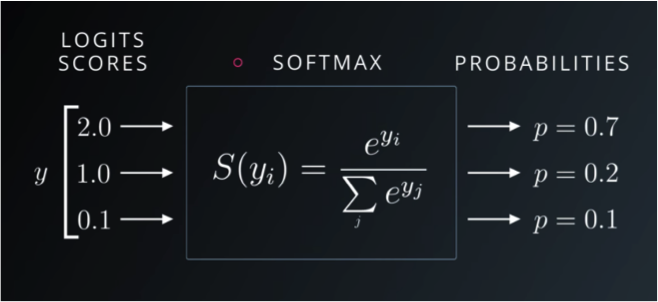
\includegraphics[width=0.75\textwidth]{images/softmax}
  \caption{ Softmax function (taken from~\cite{hinton13}) }
  \label{fig:softmax}
\end{figure}

As seen on the \fref{fig:softmax} function, softmax can take any kind of scores and turn them into proper probabilities. Because proper probabilities sum to one, results can be interpreted in the following manner: they will be more accurate when resulting scores are large that is to say close to one and consequently it will be interpreted as low when the results are relatively small. 


%%%%
\paragraph{Applications}

As told above Neural Networks have different classifications and each one provides a more accurate solution to a certain type of problems than the others. Because of this, only applications regarding models comprised by linear neurons are evaluated for the means of this work. Even with this simplification of the field, there are plenty of issues that this model can solve. An important factor contributing to this statement is the simplicity there is when training both single-element and multi-element linear networks~\cite{widrow94}. Nowadays it is frequent for general users of these models to attend applications such as handwriting and speech recognition, facial and image classification, among others. Also, multiple companies have used these in order to offer integrated functionalities in their devices. However, less common employments of this technology are also available. In the first place telecommunications include adaptive line equalizers and adaptive echo cancellers, and for each of these systems a single neural network is used. Likewise, industrial applications such as automotive systems implement these models to acquire active control of vibration and noise. Finally Stanford Linear Accelerator Center uses adaptive techniques to cancel disturbances, such as noise, that diminish the positioning accuracy of opposing beams of positrons and electrons in a particle collider~\cite{widrow94}. Although the last applications mentioned are not easily accessed by all users, understanding the broad area in which this technology can work is fundamental when understanding the pertinence of developing Neural Network models. 


\endinput

